\section{An Insert-Only List}\label{sec:list}

As a first concrete example of the approach outlined in Section~\ref{sec:approach}, we now show how to construct an ordered list data structure using an OpSet.
We initially consider a list that only supports insertion of list elements, and we extend the definition to support deletion in the following sections.

Let us assume that an OpSet may contain two types of operation:
$\mathrm{makeList}(\mathit{Oid})$ creates a new, empty list, and
$\mathrm{insertAfter}(\mathit{Oid}, \mathit{Previous})$ inserts a new list element.
The $\mathit{Oid}$ parameter of each constructor is the unique identifier of the operation.
The second parameter of insertAfter determines the insertion position: to insert at the head of a list, $\mathit{Previous}$ should equal the $\mathit{Oid}$ of the prior makeList operation that created the list; otherwise, $\mathit{Previous}$ is the $\mathit{Oid}$ of a prior insertAfter operation, and the new list element is placed after that existing list element.

In Section~\ref{sec:assign} we will show how to associate a value with every list element; for now, we will consider the list to be merely a sequence of operation IDs (oids).
An oid thus has a dual purpose: to identify an operation, but also to identify the list or list element created by that operation.

\subsection{Constructing a List from an OpSet}

We must now define a deterministic function that takes a set of makeList and insertAfter operations, and produces a corresponding list.
We do this by arranging the operations into a tree, and traversing the tree in a deterministic order.
The algorithm in this section is based on Attiya et al.'s timestamped insertion tree \cite{Attiya:2016kh}, which is similar to Grishchenko's causal tree \cite{Grishchenko:2014eh}.

\begin{figure}
\centering
\begin{minipage}{8cm}
\begin{align*}
\mathit{OpSet} = \{ &
    \mathrm{makeList}(0),\; \mathrm{insertAfter}(5, 0) \\ &
    \mathrm{insertAfter}(9, 5),\; \mathrm{insertAfter}(13, 0), \\&
    \mathrm{insertAfter}(14, 13),\; \mathrm{insertAfter}(15, 14), \\&
    \mathrm{insertAfter}(17, 14),\; \mathrm{insertAfter}(23, 14) \}
\end{align*}
\end{minipage}
\hspace{20pt}
\begin{minipage}{6cm}
\begin{tikzpicture}[level distance=10mm]
  \tikzstyle{edge from parent}=[draw,{Stealth[length=2.5mm]}-]
  \node {0}
    child {node {13}
      child {node {14}
        child {node {23}}
        child {node {17}}
        child {node {15}}
      }
    }
    child {node {5}
      child {node {9}}
    };
\end{tikzpicture}
\end{minipage}
\caption{OpSet and corresponding tree representation of the list [13, 14, 23, 17, 15, 5, 9].}\label{fig:list-tree}
\end{figure}

Figure~\ref{fig:list-tree} shows an example of such an OpSet.
To construct the tree, we create a node for each operation, and make each insertAfter node a child of the node it references in its $\mathit{Previous}$ parameter.
A makeList operation forms the root of this tree.
The list order is determined by a depth-first pre-order traversal of this tree, ignoring the root node, and visiting any sibling nodes in order of descending oid.

\begin{figure}
\centering
\[ \mathit{nextElem} = \{ (0, 13),\; (13, 14),\; (14, 23),\; (23, 17),\; (17, 15),\; (15, 5),\; (5, 9) \} \]
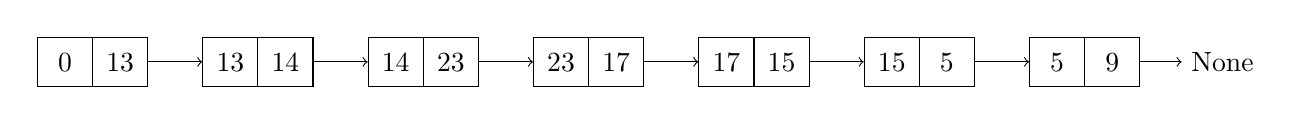
\begin{tikzpicture}
  \tikzstyle{every node}=[anchor=base,minimum width=7mm,text height=9pt,text depth=2pt]
  \matrix [column sep={7mm,between origins},nodes=draw] {
    \node (1a) {0};  & \node (1b) {13}; &&
    \node (2a) {13}; & \node (2b) {14}; &&
    \node (3a) {14}; & \node (3b) {23}; &&
    \node (4a) {23}; & \node (4b) {17}; &&
    \node (5a) {17}; & \node (5b) {15}; &&
    \node (6a) {15}; & \node (6b) {5};  &&
    \node (7a) {5};  & \node (7b) {9};  && \node (8a) [draw=none] {None}; \\
  };
  \draw [->] (1b) -- (2a);
  \draw [->] (2b) -- (3a);
  \draw [->] (3b) -- (4a);
  \draw [->] (4b) -- (5a);
  \draw [->] (5b) -- (6a);
  \draw [->] (6b) -- (7a);
  \draw [->] (7b) -- (8a);
\end{tikzpicture}
\vskip 12pt
After adding insertAfter(25, 13) to $\mathit{OpSet}$:
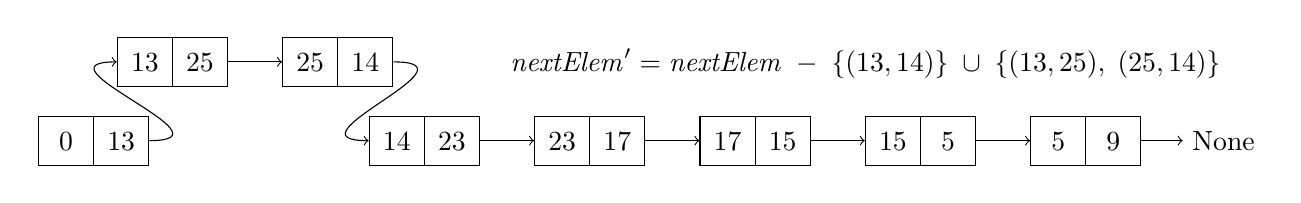
\begin{tikzpicture}
  \tikzstyle{every node}=[anchor=base,minimum width=7mm,text height=9pt,text depth=2pt]
  \node [anchor=west] at (6,1) {$\mathit{nextElem}' = \mathit{nextElem} \;-\; \{(13, 14)\} \;\cup\; \{(13, 25),\; (25, 14)\}$};
  \matrix [column sep={7mm,between origins},nodes=draw,matrix anchor=west] at (1,1) {
    \node (n1) {13}; & \node (n2) {25}; &&
    \node (n3) {25}; & \node (n4) {14}; \\
  };
  \matrix [column sep={7mm,between origins},nodes=draw,matrix anchor=west] at (0,0) {
    \node (1a) {0};  & \node (1b) {13}; &&&&&
    \node (3a) {14}; & \node (3b) {23}; &&
    \node (4a) {23}; & \node (4b) {17}; &&
    \node (5a) {17}; & \node (5b) {15}; &&
    \node (6a) {15}; & \node (6b) {5};  &&
    \node (7a) {5};  & \node (7b) {9};  && \node (8a) [draw=none] {None}; \\
  };
  \draw [->] (1b.east) .. controls (2.7,0) and (0,1) .. (n1.west);
  \draw [->] (n2) -- (n3);
  \draw [->] (n4.east) .. controls (5.8,1) and (3.2,0) .. (3a.west);
  \draw [->] (3b) -- (4a);
  \draw [->] (4b) -- (5a);
  \draw [->] (5b) -- (6a);
  \draw [->] (6b) -- (7a);
  \draw [->] (7b) -- (8a);
\end{tikzpicture}
\caption{The nextElem relation derived from the OpSet in Figure~\ref{fig:list-tree}. It describes the order of list elements similarly to a linked list.}\label{fig:next-elem}
\end{figure}

\begin{figure*}
\begin{align*}
\mathrm{isListElem}(\mathit{Oid}) \leftarrow\; &
    \mathrm{insertAfter}(\mathit{Oid}, \mathit{Parent}).\\
\mathrm{hasChild}(\mathit{Parent}) \leftarrow\; &
    \mathrm{insertAfter}(\mathit{Child}, \mathit{Parent}).\\
\mathrm{laterChild}(\mathit{Parent}, \mathit{Child2}) \leftarrow\; &
    \mathrm{insertAfter}(\mathit{Child1}, \mathit{Parent}),\;
    \mathrm{insertAfter}(\mathit{Child2}, \mathit{Parent}),\;
    \mathit{Child1} > \mathit{Child2}.\\
\mathrm{firstChild}(\mathit{Parent}, \mathit{Child}) \leftarrow\; &
    \mathrm{insertAfter}(\mathit{Child}, \mathit{Parent}),\;
    \neg\;\mathrm{laterChild}(\mathit{Parent}, \mathit{Child}).\\
\mathrm{sibling}(\mathit{Child1}, \mathit{Child2}) \leftarrow\; &
    \mathrm{insertAfter}(\mathit{Child1}, \mathit{Parent}),\;
    \mathrm{insertAfter}(\mathit{Child2}, \mathit{Parent}).\\
\mathrm{laterSibling}(\mathit{Sib1}, \mathit{Sib2}) \leftarrow\; &
    \mathrm{sibling}(\mathit{Sib1}, \mathit{Sib2}),\;
    \mathit{Sib1} > \mathit{Sib2}.\\
\mathrm{laterSibling2}(\mathit{Sib1}, \mathit{Sib3}) \leftarrow\; &
    \mathrm{sibling}(\mathit{Sib1}, \mathit{Sib2}),\;
    \mathrm{sibling}(\mathit{Sib1}, \mathit{Sib3}),\;
    \mathit{Sib1} > \mathit{Sib2},\;
    \mathit{Sib2} > \mathit{Sib3}.\\
\mathrm{nextSibling}(\mathit{Sib1}, \mathit{Sib2}) \leftarrow\; &
    \mathrm{laterSibling}(\mathit{Sib1}, \mathit{Sib2}),\;
    \neg\;\mathrm{laterSibling2}(\mathit{Sib1}, \mathit{Sib2}).\\
\mathrm{hasNextSibling}(\mathit{Sib1}) \leftarrow\; &
    \mathrm{laterSibling}(\mathit{Sib1}, \mathit{Sib2}).\\
\mathrm{nextSiblingAnc}(\mathit{Start}, \mathit{Next}) \leftarrow\; &
    \mathrm{nextSibling}(\mathit{Start}, \mathit{Next}).\\
\mathrm{nextSiblingAnc}(\mathit{Start}, \mathit{Next}) \leftarrow\; &
    \neg\;\mathrm{hasNextSibling}(\mathit{Start}),\;
    \mathrm{insertAfter}(\mathit{Start}, \mathit{Parent}),\;
    \mathrm{nextSiblingAnc}(\mathit{Parent}, \mathit{Next}).\\
\mathrm{hasSiblingAnc}(\mathit{Start}) \leftarrow\; &
    \mathrm{nextSiblingAnc}(\mathit{Start}, \mathit{Next}).\\
\mathrm{nextElem}(\mathit{Prev}, \mathit{Next}) \leftarrow\; &
    \mathrm{firstChild}(\mathit{Prev}, \mathit{Next}).\\
\mathrm{nextElem}(\mathit{Prev}, \mathit{Next}) \leftarrow\; &
    \mathrm{isListElem}(\mathit{Prev}),\;
    \neg\;\mathrm{hasChild}(\mathit{Prev}),\;
    \mathrm{nextSiblingAnc}(\mathit{Prev}, \mathit{Next}).\\

\end{align*}
\caption{Datalog rules for an ordered list (insertion only).}\label{fig:list-insert-datalog}
\end{figure*}

More formally, 

Figure~\ref{fig:list-insert-datalog} gives a Datalog query that expresses this traversal.
For readers who are unfamiliar with Datalog, it can informally be read as follows: if all predicates on the right-hand side of an arrow can be satisfied by some variable assignment, then we can conclude that the left-hand side is also true.
Later rules build upon earlier rules to create more complex constructions.
